\documentclass[tikz,border=2mm]{standalone}
\usepackage{amsmath,amssymb}
\usetikzlibrary{arrows.meta,positioning}
\newcommand{\tikzsetnextfilename}[1]{}
% Reusable primitives for partition-labelled growth diagrams.
% Coordinates refer to grid vertices; cell entries use the southwest corner.

\tikzset{
  growth diagram grid/.style={draw=black!60, line width=0.65pt},
  growth diagram highlight/.style={fill=black!8},
  growth diagram vertex/.style={
    fill=white,
    inner sep=1.5pt,
    rounded corners=1pt,
    font=\small
  },
  growth diagram entry/.style={
    font=\small,
    text=black!70
  }
}

% \growthDiagramGrid[options]{columns}{rows}
\newcommand{\growthDiagramGrid}[3][]{%
  \draw[growth diagram grid,#1] (0,0) grid (#2,#3);%
}

% \growthDiagramHighlight[options]{x}{y}
\newcommand{\growthDiagramHighlight}[3][]{%
  \path[growth diagram highlight,#1] (#2,#3) rectangle ++(1,1);%
}

% \growthDiagramEntry[options]{x}{y}{entry}
\newcommand{\growthDiagramEntry}[4][]{%
  \node[growth diagram entry,#1] at ({#2+0.5},{#3+0.5}) {#4};%
}

% \growthDiagramVertex[options]{x}{y}{partition}
\newcommand{\growthDiagramVertex}[4][]{%
  \node[growth diagram vertex,#1] at (#2,#3) {$#4$};%
}


\begin{document}

\tikzsetnextfilename{rsk-growth-diagram}
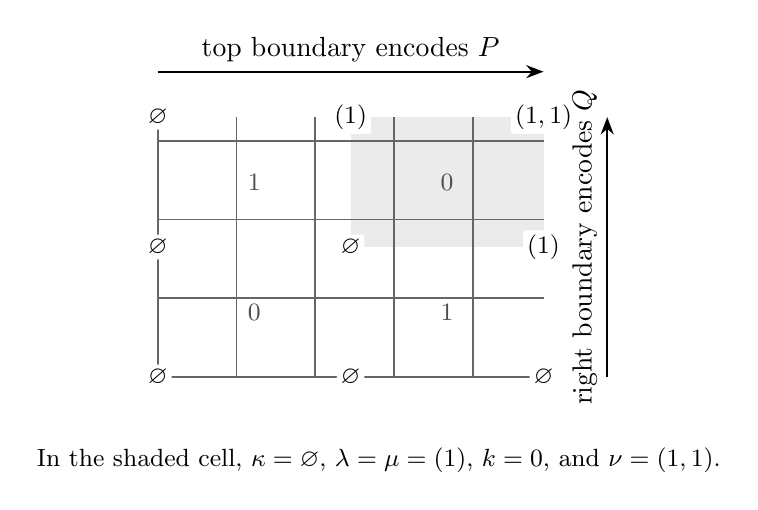
\begin{tikzpicture}[x=2.45cm,y=1.65cm]
  \growthDiagramHighlight{1}{1}
  \growthDiagramGrid{2}{2}

  \growthDiagramEntry{0}{0}{$0$}
  \growthDiagramEntry{1}{0}{$1$}
  \growthDiagramEntry{0}{1}{$1$}
  \growthDiagramEntry{1}{1}{$0$}

  \growthDiagramVertex{0}{0}{\varnothing}
  \growthDiagramVertex{1}{0}{\varnothing}
  \growthDiagramVertex{2}{0}{\varnothing}
  \growthDiagramVertex{0}{1}{\varnothing}
  \growthDiagramVertex{1}{1}{\varnothing}
  \growthDiagramVertex{2}{1}{(1)}
  \growthDiagramVertex{0}{2}{\varnothing}
  \growthDiagramVertex{1}{2}{(1)}
  \growthDiagramVertex{2}{2}{(1,1)}

  \draw[-{Stealth[length=2.2mm]},line width=0.7pt]
    (0,2.35) -- (2,2.35)
    node[midway,above] {top boundary encodes $P$};
  \draw[-{Stealth[length=2.2mm]},line width=0.7pt]
    (2.33,0) -- (2.33,2)
    node[midway,right,rotate=90,anchor=south] {right boundary encodes $Q$};

  \node[below=3mm of current bounding box.south,align=center,font=\small]
    {In the shaded cell,
     $\kappa=\varnothing$, $\lambda=\mu=(1)$, $k=0$, and
     $\nu=(1,1)$.};
\end{tikzpicture}

\end{document}
